\documentclass[11pt, openany, a4paper]{article}

\usepackage{etex}
\usepackage{fullpage}
\usepackage{pstricks,pstricks-add,pst-math,pst-xkey}
\usepackage[frenchb]{babel}
%\usepackage{slashbox}
\usepackage{graphicx}
\usepackage{amsmath,amssymb,amstext,amsthm}
%\usepackage{comment}
\usepackage[utf8]{inputenc}
\usepackage[OT1]{fontenc}
\usepackage{pgf,tikz}
\usepackage{pgfplots}
\usepackage{floatpag}
\usepgfmodule{shapes}
\usetikzlibrary{arrows,patterns}
\usepackage{floatflt}
\usepackage{import}
\usepackage{xcolor}
\usepackage{natbib}
%\usepackage{fourier-orns}

\newcounter{moncompteur}
\newtheorem{q}[moncompteur]{ \textbf{Question}}{}
\newtheorem{prop}[moncompteur]{ \textbf{Proposition}}{}
\newtheorem{df}[moncompteur]{ \textbf{Définition}}{}
\newtheorem*{df*}{ \textbf{Définition}}{}
\newtheorem{rem}[moncompteur]{ \textbf{Remarque}}{}
\newtheorem{theo}[moncompteur]{ \textbf{Théorème}}{}
\newtheorem{conj}[moncompteur]{ \textbf{Conjecture}}{}
\newtheorem{cor}[moncompteur]{ \textbf{Corollaire}}{}
\newtheorem{lm}[moncompteur]{ \textbf{Lemme}}{}
%\newtheorem{nota}[moncompteur]{ \textbf{Notation}}{}
%\newtheorem{conv}[moncompteur]{ \textbf{Convention}}{}
\newtheorem{exa}[moncompteur]{ \textbf{Exemple}}{}
\newtheorem{ex}[moncompteur]{ \textbf{Exercice}}{}
%\newtheorem{app}[moncompteur]{ \textbf{Application}}{}
%\newtheorem{prog}[moncompteur]{ \textbf{Algorithme}}{}
%\newtheorem{hyp}[moncompteur]{ \textbf{Hypothèse}}{}
\newenvironment{dem}{\noindent\textbf{Preuve}\\}{\flushright$\blacksquare$\\}
\newcommand{\cg }{[\kern-0.15em [}
\newcommand{\cd}{]\kern-0.15em]}
\newcommand{\R}{\mathbb{R}}
\newcommand{\K}{\mathbb{K}}
\newcommand{\N}{\mathbb{N}}
\newcommand{\Z}{\mathbb{Z}}
\newcommand{\C}{\mathbb{C}}
\newcommand{\U}{\mathbb{U}}
\newcommand{\Q}{\mathbb{Q}}
\newcommand{\B}{\mathbb{B}}
\newcommand{\card}{\mathrm{card}}
\newcommand{\norm}[1]{\left\lVert#1\right\rVert}
\pgfplotsset{compat=newest}
\newcommand{\La}{\mathcal{L}}
\newcommand{\Ne}{\mathcal{N}}
\newcommand{\D}{\mathcal{D}}
\newcommand{\Ss}{\textsc{safestay}}
\newcommand{\Sg}{\textsc{safego}}
\newcommand{\M}{\textsc{move}}
\newcommand{\E}{\mathcal{E}}
\newcommand{\V}{\mathcal V}
\setlength{\parindent}{0pt}
\newcommand{\myrightleftarrows}[1]{\mathrel{\substack{\xrightarrow{#1} \\[-.6ex] \xleftarrow{#1}}}}
\newcommand{\longrightleftarrows}{\myrightleftarrows{\rule{1cm}{0cm}}}

\definecolor{bleuclair}{rgb}{0.75,0.75,1.0}
\newcommand{\ANNOT}[1]{
  ~\linebreak
  \centerline{
    %{\Huge{\danger}}
    \large\fcolorbox{black}{bleuclair}{
      \begin{minipage}[h]{.8\linewidth}
      #1
      \end{minipage}
    }
    %{\Huge{\danger}}
  }
}

\newcommand\tikzmark[1]{%
  \tikz[overlay,remember picture,baseline] 
  \node[anchor=base](#1){};}

\newcommand\MyLine[3][]{%
  \begin{tikzpicture}[overlay,remember picture]
    \draw[#1] (#2.north west) -- (#3.south east);
  \end{tikzpicture}}


\graphicspath{{.}}
\newcommand{\e}[1]{$\times 10^{#1}$}
\begin{document}

\title{Algorithmes pour les systèmes de recommandation : un comparatif}
\date{}
\maketitle
\section*{Introduction}

Définition : collaborative filtering

Position du problème : 
Attentes vis-à-vis des algorithmes (précision/temps de réponse/ajout rapide d'un rating/cold start...)

Efficacité peut varier selon la forme du jeu de données (sparsity...)

Objectif : Implémenter (en Matlab) et comparer différents algorithmes en terme de précision et de temps d'exécution sur différents jeux de données, mettre en relief les compromis à faire.

\section{Les algorithmes utilisés}
	\subsection{Algorithmes témoins}
		Algorithmes naïfs servant de point de comparaison : 
			\begin{itemize}
				\item{"Witness" : Estimer tous les ratings inconnus par la moyenne de tous les ratings possibles}
				\item{"PerUserAverage" : Estimer tous les ratings inconnus pour un utilisateur donné par la moyenne des ratings connus qu'il a attribués}
				\item{"BiasFromMean" : Estimer la note donnée par un utilisateur à un objet en fonction de sa moyenne, mais aussi des écarts entre les notes attribuées à l'objet et les moyennes des utilisateurs qui l'ont noté}
				\item{"UnbiasedWitness" : Retirer les biais comme dans le cours, estimer tous les ratings inconnus par $0$, remettre les biais}
			\end{itemize}
	\subsection{SVD}
		Variantes sur la question bonus du DM (comment traiter les trous dans la matrice, avec ou sans traitement des biais...).
		\begin{itemize}
			\item{"ShiftSVD" : translater la matrice pour avoir $0$ de moyenne, SVD, retranslater}
			\item{"UnbiasedSVD" : enlever les biais, SVD, remettre les biais}
		\end{itemize}
	\subsection{Algorithmes Slope One}
		Prédicteur affine, en imposant une pente de 1. Pour tout couple d'objet, on définit une déviation de l'un par rapport à l'autre, un peu comme la mesure de similarité cosinus, mais en beaucoup plus simple (linéaire). La prédiction de la note attribuée à un objet s'obtient alors en ajoutant la moyenne de l'utilisateur et la moyenne des déviations de l'objet aux autres objets notés par l'utilisateur. D'où un prédicteur de forme $f(x)=x+b$.
	
		
		
		Calculs simples. Possibilité de garder les déviations en mémoire : traitement d'une requête très rapide. De plus, ces déviations peuvent même être mises à jour sans tout recalculer quand on ajoute un rating.
		
		\`A quel point est-ce moins précis que d'autres algos plus sophistiqués ?
		
		Variante : donner plus de poids aux déviations des paires d'objets qui ont été notés tous deux à la fois par un grand nombre d'utilisateurs, car elles sont plus fiables.
		
		Algorithmes tirés de \cite{Lemire2007}.
	\subsection{Algorithmes par similarité cosinus}
		Implémentation des algorithmes vus en cours : "itemCosSimilarity", "userCosSimilarity".
		
	\subsection{Analyse en composantes principales : algorithme Eigentaste\cite{Goldberg2001}}
		Idée : s'appuyer sur un petit sous-ensemble d'objets notés par tous les utilisateurs (\emph{gauge set}) pour projeter un utilisateur sur un espace de petite dimension puis estimer ses notes à partir de celles de ses voisins au sens d'un algorithme de clustering. Eigentaste ne s'applique donc qu'aux jeux de données comprenant un tel gauge set, comme le jeu de données Jester.
		
		Notons $R$ la matrice $(n\times m)$ des ratings, $G$ le gauge set, $k=|G|$.
		
		On commence par normaliser les ratings des utilisateurs sur les objets du gauge set : la qualité objective d'un objet importe peu ici car on cherche à obtenir des informations sur les ressemblances entre utilisateurs par analyse de composantes principales.
		
		Pour tout objet $j$, on calcule donc $\mu_j=\sum_{i=1}^n r_{ij}$ la note moyenne de cet objet, et $$\sigma_j^2 = \frac{1}{n-1} \sum_{i=1}^{n} (r_{ij} - \mu_j)$$ sa variance.
		
		On obtient alors la matrice $A$ (de taille $k\times k$) des ratings normalisés sur le gauge set : $a_{ij} = \frac{r_{ij}-\mu_j}{\sigma_j}$.
		
		On pose $C=\frac{1}{n-1} A^T A$ (matrice de corrélation de Pearson). Elle est symétrique définie positive, on note $\Lambda$ la matrice diagonale contenant ses valeurs propres triées par ordre décroissant et $E$ la matrice orthogonale de vecteurs propres associée. On a $EE^T = Id$, $C = E\Lambda E^T$.
		
		On peut alors projeter les vecteurs correspondant aux utilisateurs sur un petit sous-espace (de dimension $v$) contenant l'essentiel de la variance en posant $X=AE^T_v$. 
		En particulier, pour $v=k$, on a $C_X = \frac{1}{n-1} X^T X = ECE^T = \Lambda$ diagonale : les vecteurs sont décorrélés.
		On prend $v=2$ dans la suite.
		
			\begin{figure}[ht!]
				\centering
				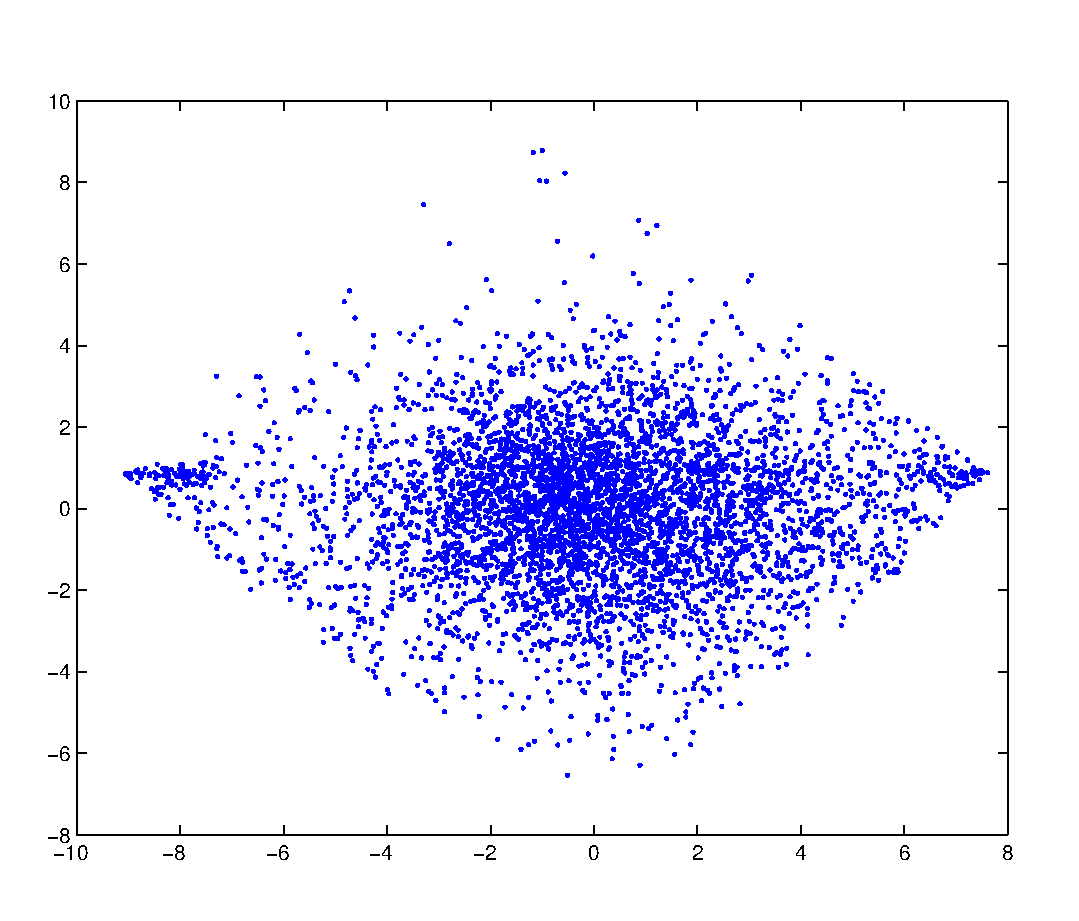
\includegraphics[height=120mm]{eigentaste_proj_cropped.pdf}
				\caption{Projection pour $v=2$ sur un sous-ensemble du jeu de données Jester}
			\end{figure}
			
		On regroupe ensuite les utilisateurs proches par amas en utilisant un algorithme de clustering (\cite{Goldberg2001} utilise un algorithme récursif rectangulaire, nous avons utilisé les fonctions Matlab \emph{linkage} et \emph{cluster} dans notre implémentation).
		
		On estime ensuite un rating de l'utilisateur $i$ sur l'objet $j$ par la moyenne des notes pour $j$ des utilisateurs se trouvant dans le même cluster que $i$.
		
		\medskip
						
		Cet algorithme a l'inconvénient de ne s'appliquer qu'à certains jeux de données : pour ajouter un nouvel utilisateur, il faut d'abord lui faire noter l'intégralité du gauge set (typiquement une dizaine d'objets). De plus, on ne peut rien dire sur un utilisateur seul dans son amas : le démarrage à froid pose problème.
		
		En revanche, ajouter un utilisateur qui a noté le gauge set est peu coûteux en termes de temps de calcul : on peut lui recommander rapidement des objets dès qu'on a choisi son cluster, l'idée étant de ne pas modifier immédiatement les projections des anciens utilisateurs mais plutôt de tout remettre à jour périodiquement.
		
		Dans la suite, on se propose de comparer Eigentaste avec d'autres algorithmes de recommandation en termes de précision et de temps de calcul, sur le jeu de données Jester.
		
		
		
		
\section{Observations expérimentales}
	\subsection{Jeux de données}
		\begin{itemize}
			\item{Matrice de la question bonus du DM (pleine, on observe seulement une certaine fraction des ratings)}
			\item{Jeu de données Jester (ratings d'une centaine de blagues, dix blagues sont notées par toutes les utilisateurs) utilisé pour Eigentaste.}
			\item{Jeu de données plus grand (MovieLens) pour mesurer les difficultés liées aux temps d'exécutions dans des conditions plus réalistes ?}
		\end{itemize}
	\subsection{Mesures d'erreur}
	
		\begin{figure}[ht!]
			\centering
			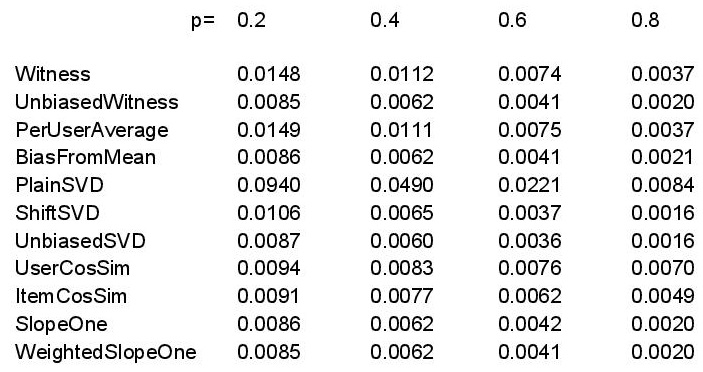
\includegraphics[width=0.8\linewidth]{resultatsPrerapport.jpg}
		\end{figure}
		Sur la matrice du DM, on obtient ce tableau d'erreurs MSE pour différentes valeurs de p :
		
		Eigentaste et quelques autres ne sont pas encore implémentés.
		à venir aussi : une autre mesure d'erreur, et des mesures sur les autres jeux de données.
		
		L'algorithme simple "BiasFromMean" obtient d'excellents résultats !  Les variantes de Slope One obtiennent aussi des résultats très comparables aux algorithmes SVD plus complexes à mettre en œuvre.
	\subsection{Temps d'exécution}
	
		\begin{figure}[ht!]
			\centering
			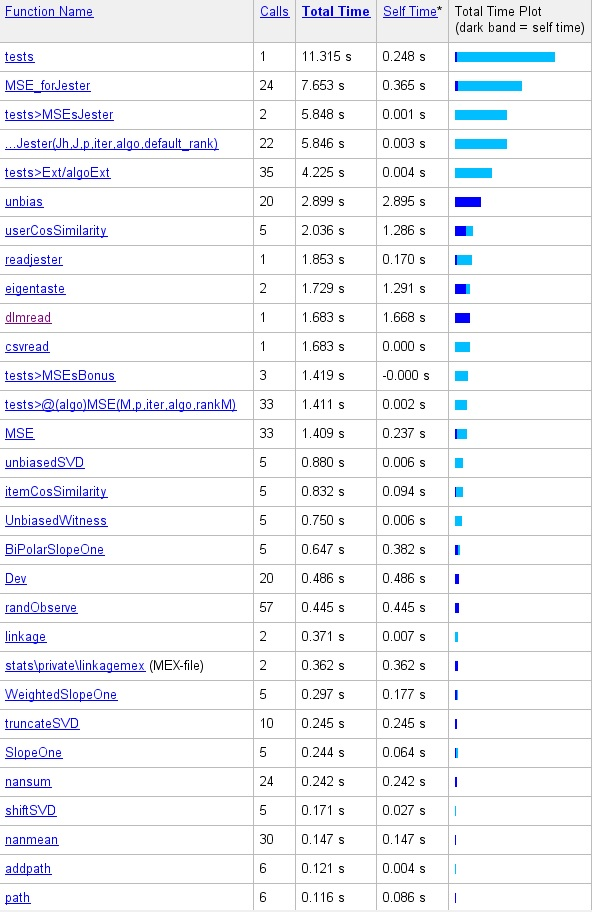
\includegraphics[height=120mm]{times.jpg}
			\caption{Profiling fourni par Matlab}
		\end{figure}
		

		Les algorithmes qui enlèvent et remettent les biais comme dans le cours s'exécutent beaucoup plus lentement : il faut inverser une matrice creuse, et on n'a pas réussi à vectoriser une partie du calcul de l'argmin pour les biais. Il faudra essayer l'expression plus naïve des biais et voir ce qu'on gagne en temps/perd en précision.
		
		Il faut aussi tenir compte du fait que certains algos (Slope One oui, SVD non) calculent des choses "une fois pour toutes", et c'est rapide d'ajouter un utilisateur et/ou de faire une requête.
		
\bibliographystyle{plain}
\bibliography{biblio}

\end{document}